\section{Filter}


\subsection{Grundtypen}{291}

Filter sind mehrheitlich \textbf{frequnezselektive, lineare Netzwerke}, welche gewisse Frequenzbereiche übertragen
und andere dämpfen. Die fünf \textbf{frequnezselektiven Grundtypen} sind: 

\begin{minipage}[t]{0.25\columnwidth}
    \begin{itemize}
        \item Tiefpass (TP)
        \item Hochpass (HP)
    \end{itemize}
\end{minipage}
\hfill
\begin{minipage}[t]{0.35\columnwidth}
    \begin{itemize}
        \item Bandpass (BP)
        \item Bandsperre, Notch (BS)
    \end{itemize}
\end{minipage}
\hfill
\begin{minipage}[t]{0.25\columnwidth}
    \begin{itemize}
        \item Allpass
    \end{itemize}
\end{minipage}


% \subsection{Filterbauarten}{292}

% \textrightarrow\ Siehe Skript S. 292

% \begin{tabular}{|l|l|l|l|}
%     \hline
%     \multirow{7}{*}{\rotatebox[origin=c]{90}{zeitdiskret}}         & \multirow{7}{*}{aktiv}    & \multirow{3}{*}{\begin{tabular}[c]{@{}l@{}}diskrete\\ Werte\end{tabular}}         & Filter mit Signalprozessor           \\ \cline{4-4} 
%                                       &                            &                                                                                   & Filter mit Gate Logic                \\ \cline{4-4} 
%                                       &                            &                                                                                   & etc.                                 \\ \cline{3-4} 
%                                       &                            & \multirow{4}{*}{\begin{tabular}[c]{@{}l@{}}analoge\\ Werte\end{tabular}}          & SC-Filter (Switched Capacitor)       \\ \cline{4-4} 
%                                       &                            &                                                                                   & SI-Filter (Switched Current)         \\ \cline{4-4} 
%                                       &                            &                                                                                   & N-Pfad Filter                        \\ \cline{4-4} 
%                                       &                            &                                                                                   & etc.                                 \\ \hline
%     \multirow{16}{*}{\rotatebox[origin=c]{90}{kontinurierlich}}    & \multirow{5}{*}{aktive RC} & \multirow{5}{*}{\begin{tabular}[c]{@{}l@{}}konz. \\ Bauteile\end{tabular}}        & 'Simultion' von LC-Filtern           \\ \cline{4-4} 
%                                       &                            &                                                                                   & Gekoppelte Filterstrukturen          \\ \cline{4-4} 
%                                       &                            &                                                                                   & Filter Parallelform                  \\ \cline{4-4} 
%                                       &                            &                                                                                   & Filter in Kaskadenbauweise           \\ \cline{4-4} 
%                                       &                            &                                                                                   & etc.                                 \\ \cline{2-4} 
%                                       & \multirow{11}{*}{passiv}   & \multirow{4}{*}{\begin{tabular}[c]{@{}l@{}}verteilte\\ Bauteile\end{tabular}}     & SAW-Filter (Surfaec Acoustic Wave)   \\ \cline{4-4} 
%                                       &                            &                                                                                   & Hohlraumresonatoren (Topfkreisfilter \\ \cline{4-4} 
%                                       &                            &                                                                                   & Leisutngsfilter                      \\ \cline{4-4} 
%                                       &                            &                                                                                   & etc.                                 \\ \cline{3-4} 
%                                       &                            & \multirow{7}{*}{\begin{tabular}[c]{@{}l@{}}konzentrierte\\ Bauteile\end{tabular}} & Keramische Filter                    \\ \cline{4-4} 
%                                       &                            &                                                                                   & Quarz-Filter                         \\ \cline{4-4} 
%                                       &                            &                                                                                   & RLC-Filter                           \\ \cline{4-4} 
%                                       &                            &                                                                                   & RC-Filter                            \\ \cline{4-4} 
%                                       &                            &                                                                                   & LC-Filter                            \\ \cline{4-4} 
%                                       &                            &                                                                                   & LC-Filter mit Quarz                  \\ \cline{4-4} 
%                                       &                            &                                                                                   & etc.                                 \\ \hline
% \end{tabular}


\subsection[Frequnezgang H(jimg omega) -- Übertragungsfunktion H(s)]{Frequnezgang $H(\jimg \omega)$ -- Übertragungsfunktion $H(s)$}{294}

Für den Frequnezgang $H(\jimg \omega)$ und die Übertragungsfunktion $H(s)$ gelten die folgenden Zusammenhänge

$$ | H(\jimg \omega) |^2 = H(\jimg \omega) \cdot H^*(\jimg \omega) = H(\jimg \omega) \cdot H(- \jimg \omega) = H(s) \cdot H(-s) \Big|_{s = \jimg \omega} $$
$$ H(s) \cdot H(-s) = | H(\jimg \omega) |^2 \Big|_{\omega^2 = -s^2} $$
\textbf{Hinweis:} $| H(\jimg \omega) |^2$ ist immer eine Funktion in $\omega^2$, da der Amplitudengang eine gerade Funktion ist!

\vspace{0.2cm}

Da in der Praxis \textbf{jeweils nur $\bm{H(s)}$ interessant} ist, muss $H(s)$ aus $| H(\jimg \omega) |^2$ 'isoliert' werden. 
Dies ist durch den folgenden Zusammenhang möglich.

$$ \boxed{ \underbrace{ \frac{N(s)}{D(s)} }_{H(s)} \cdot  \underbrace{ \frac{N(-s)}{D(-s)} }_{H(-s)} = | H(\jimg \omega) |^2 \Big|_{\omega^2 = -s^2} } $$
\textbf{Hinweis:} $D(s)$ muss aus Stabilitätsgründen ein Hurwitz-Polynom sein!


\subsection{Approximation im Frequnezbereich}

Die wichtigste Aufgabe der Filtertheorie ist die \textbf{Bestimmung der Übertragungsfunktion, die einen vorgegebenen 
Frequenzgang gewährleistet.} Zuerst soll der \textbf{Amplitudengang} $| H(\jimg \omega) |$ im Frequnezbereich approximiert werden.
Der vorgeschriebene Phasengang wird dann allenfalls mit zusätzlichen Allpass-Filtern erreicht. 


\subsubsection{Toleranzschema (Stempel und Matritze) -- Filterspezifikation}
\label{Toleranzschema}

\begin{minipage}[c]{0.48\columnwidth}
    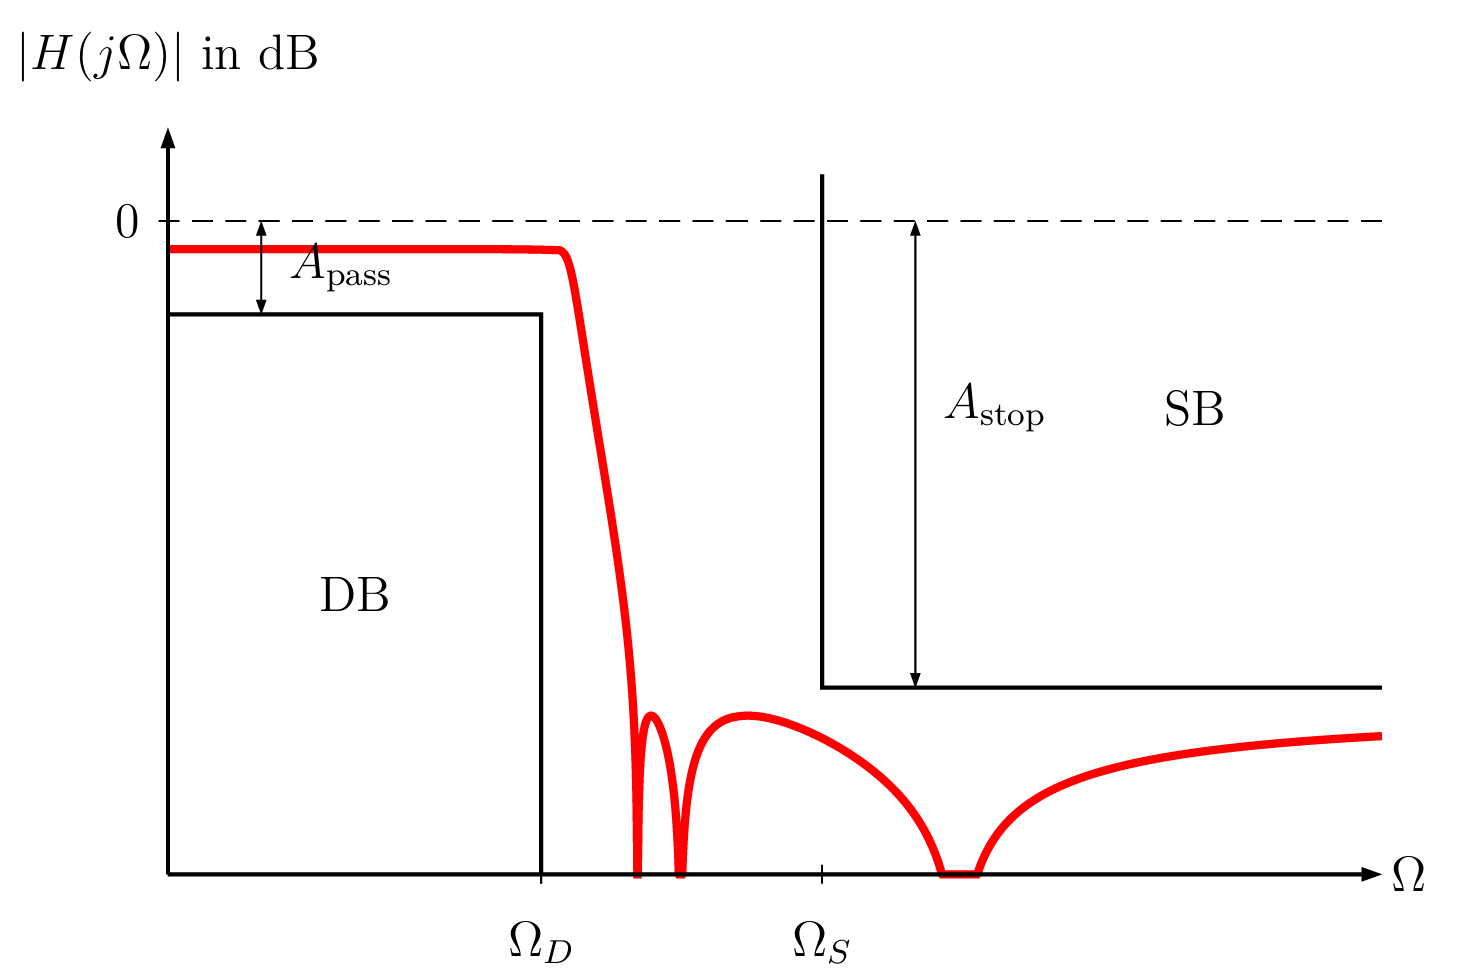
\includegraphics[width=\columnwidth]{images/filter_toleranzschema.png}
\end{minipage}
\hfill
\begin{minipage}[c]{0.48\columnwidth}
    Die Anforderungen an ein Filter werden häufig im \textbf{Toleranzschema beschrieben}. Dieses steht jeweils 'auf dem Kopf'.

    \begin{itemize}
        \item Im \textbf{Durchlassbereich (DB)} bestimmt der Stempel die maximal zulässige \textbf{Dämpfung} $A_{\rm max}$
        \item Im \textbf{Sperrbereich (SB)} bestimmt die Matritze die minimal nötige \textbf{Dämpfung} $A_{\rm min}$
    \end{itemize}
\end{minipage}

$$\boxed{ A_{\deci \bel}(\omega) = 10 \cdot \log \Biggl( \frac{1}{|H(\omega)|^2} \Biggr) = - 20 \cdot \log \bigl(|H(\omega)| \bigr) 
    \quad \textrightarrow\ \text{Dämpfung!} } $$


\subsubsection{Frequenznormierung}
 
Um möglist kompakte \textbf{Tabellen} zu haben, wird auf Frequenzen normiert. Grundsätzlich kann auf eine beliebige Frequenz normiert
werden. Allerdings gilt grundsätzlich:

\begin{itemize}
    \item \textbf{HP / TP:} Normierung bezüglich \textbf{Grenzfrequenz} des Durchlassbereichs $\omega_r = \omega_D$
    \item BP / BS: Normierung bezüglich der Mittenfrequenz $\omega_r = \omega_m$
\end{itemize}
\vspace{0.2cm}

\begin{minipage}[c]{0.48\columnwidth}
    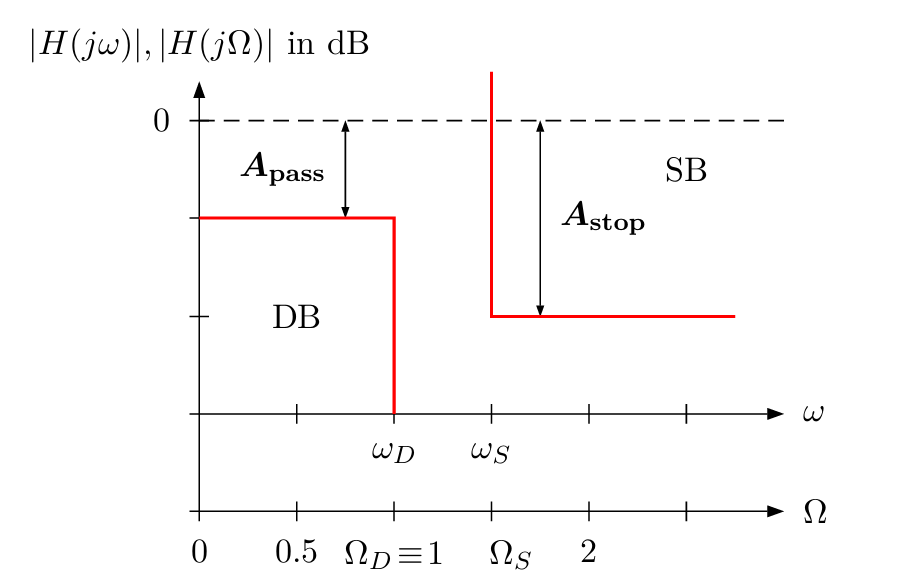
\includegraphics[width=\columnwidth]{images/filter_toleranzschema_frequenznormierung.png}
\end{minipage}
\hfill
\begin{minipage}[c]{0.48\columnwidth}
    \begin{center}
       \textbf{\myul{Normierte Grössen}}  
    \end{center}

    \vspace{-0.3cm}
    \begin{minipage}[c]{0.3\columnwidth}
        $$ \boxed{ S = \frac{s}{\omega_r}} $$
    \end{minipage}
    \hfill
    \begin{minipage}[c]{0.3\columnwidth}
        $$ \boxed{ \Omega = \frac{\omega}{\omega_r}} $$
    \end{minipage}
    \hfill
    \begin{minipage}[c]{0.3\columnwidth}
        $$ \boxed{ \sigma' = \frac{\sigma}{\omega_r}} $$ 
    \end{minipage}

    \vspace{0.2cm}
    \textbf{Hinweis:} Zur Entnormierung wird jeweils $S$ in der normierter Funktion durch $\frac{s}{\omega_r}$ ersetzt.
\end{minipage}


\subsection{Ideales Tiefpassfilter}{297}

\begin{minipage}[c]{0.48\columnwidth}
    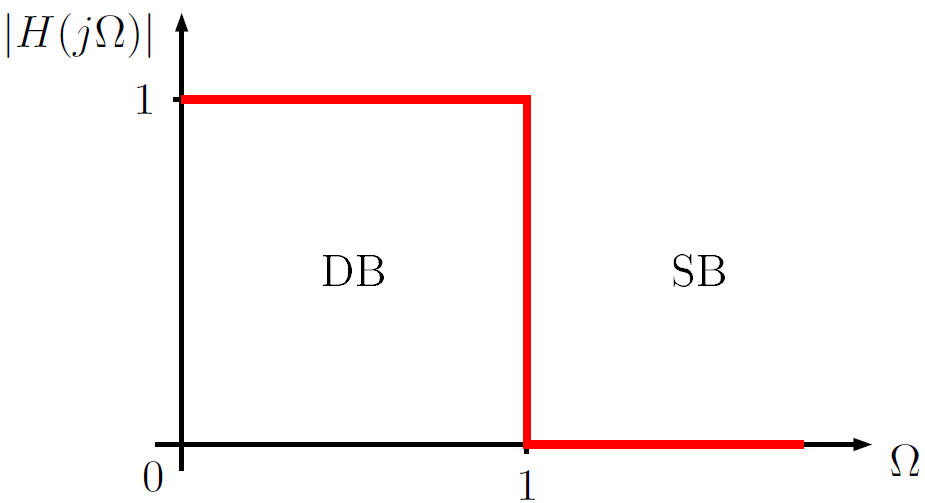
\includegraphics[width=\columnwidth]{images/filter_toleranzschema_idealer_tiefpass.png}

    \begin{itemize}
        \item DB: keine Dämpfung
        \item SB: kein Ausgangssignal
    \end{itemize}
\end{minipage}
\hfill
\begin{minipage}[c]{0.42\columnwidth}
    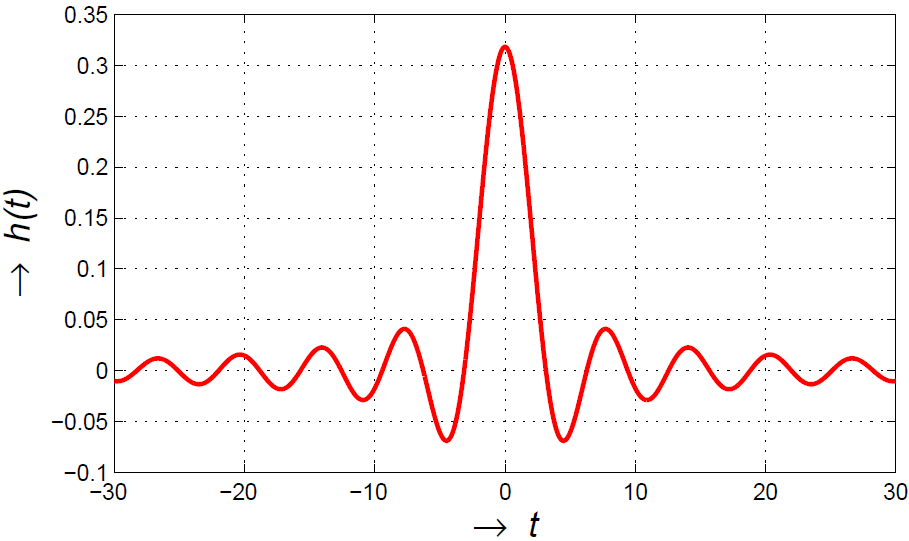
\includegraphics[width=\columnwidth]{images/filter_impulsantwort_idealer_tiefpass.png}
    
    \begin{itemize}
        \item Akausale Impulsantwort $h(t)$
    \end{itemize}
\end{minipage}

\vspace{0.2cm}
\textrightarrow\ Ideales Tierpass ist physikaltisch nicht realisierbar. \textrightarrow\ \textbf{Approximationen}


\subsection[Amplitudengang mit char. Funktion K(Omega2)]{Amplitudengang mit char. Funktion $K(\Omega^2)$}
\label{Amplitudengang mit char. Funktion}

Um Wurzelausdrücke zu vermeiden, wird der folgenden Ansatz verwendet
$$ \boxed{ | H(\jimg \Omega) |^2 = \frac{1}{1 + K(\Omega^2)}} $$

Im Fall des (idealen) Tiefpasses gilt füt die charakteristische Funktion $K(\Omega^2)$

\begin{tabular}{l r l l}
    Durchlassbereich (DB)   & $0 \leq K(\Omega^2) \ll 1$    & für $0 \leq \Omega < 1$   & \textrightarrow\ $| H(\jimg \Omega) |^2 \approx 1$ \\
    Sperrbereich (SB)       & $K(\Omega^2) \gg 1$           & für $ \Omega > 1$         & \textrightarrow\ $| H(\jimg \Omega) |^2 \approx 0$ \\   
\end{tabular}


\subsection{Approximation mittels kritisch-gedämpfter Filter}{299}

Tiefpassfilter $n.$ Ordnung mit kritischer Dämpfung haben jeweilen einen $\bm{n}$\textbf{-fachen Pol} auf der \textbf{negativen}
$\sigma$-Achse.

\begin{itemize}
    \item Impuls- und Sprungantwort können nicht oszillieren
    \item Geringe Flankensteilheit im Übergangsbereich
\end{itemize}
\vspace{0.2cm}

Die Übertragungsfunktion $H(s)$ ergibt sich als:

\begin{minipage}[c]{0.48\columnwidth}
    $$ \boxed{ H(s) = \frac{1}{\Big( 1 + \frac{s}{\omega_c} \Big)^n} } $$
\end{minipage}
\hfill
\begin{minipage}[c]{0.48\columnwidth}
    \begin{tabular}{ll}
        $n$         & Ordnung des Filters \\
        $\omega_c$  & $3 \, \deci \bel$-Punkt jedes der $\bm{n}$ \textbf{Teilfilter}
    \end{tabular}
\end{minipage}

\vspace{0.2cm}
Will man bei der Kreisfrequenz $\omega_D$ eine Dämpfung von $\alpha \, \deci \bel$ haben, so muss $\omega_c$ (der $n$ identischen
Teilfilter) gewählt werden als
$$ \boxed{ \omega_c = \frac{\omega_D}{\sqrt{10^{\frac{\alpha}{10 \cdot n}} -1}} } $$ 


\subsubsection{Eigenschaten kritisch-gedämpfte Filter}

\begin{itemize}
    \item Alle Pole am \textbf{gleichen Ort} auf negativer $\sigma$-Achse \textrightarrow\ Allpolfilter
    \item Für $\Omega = 0$ ist für sämtliche $n$: $|H(0)| = H_{\rm max} = 1$
    \item Für $\Omega = 1$ ist für sämtliche $n$: $|H(\jimg)| = \frac{H_{\rm max}}{\sqrt{2}} = \frac{1}{\sqrt{2}}$
        \textrightarrow\ $3 \, \deci \bel$ Dämpfung
    \item Für $\Omega \gg 1$ wird $|H(\jimg \Omega)| \approx \frac{1}{\Omega^n}$ \textrightarrow\ $\bm{- n \cdot 20 \, \deci \bel /}$ \textbf{Dekade}
    \item Amplitudengang bei $\Omega = 0$ maximal flach, da alle Ableitungen $=0$ sind
    \item Amplitudengang ist streng-monoton fallend \textrightarrow\ keine Welligkeit
    \item Pole verschieben sich bei höherer Ordnung in Richtung imaginäre Achse
    \item Gruppenlaufzeit konstant bis $\omega_D$
\end{itemize}


\begin{minipage}[c]{0.4\columnwidth}
    \begin{center}
        \textbf{\myul{Amplitudengänge}}
    \end{center}
    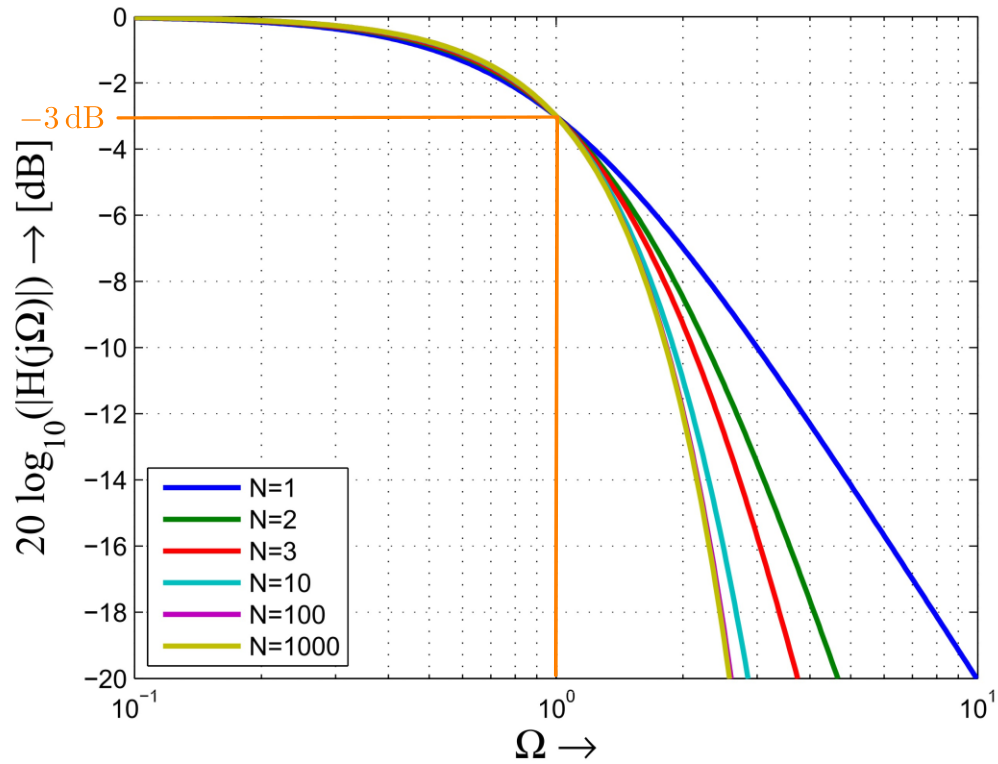
\includegraphics[width=\columnwidth]{images/filter_kritisch_gedaempft_normierter_amplitudengang.png}
\end{minipage}
\hfill
\begin{minipage}[c]{0.4\columnwidth}
    \begin{center}
        \textbf{\myul{Pol-Lagen}}
    \end{center}
    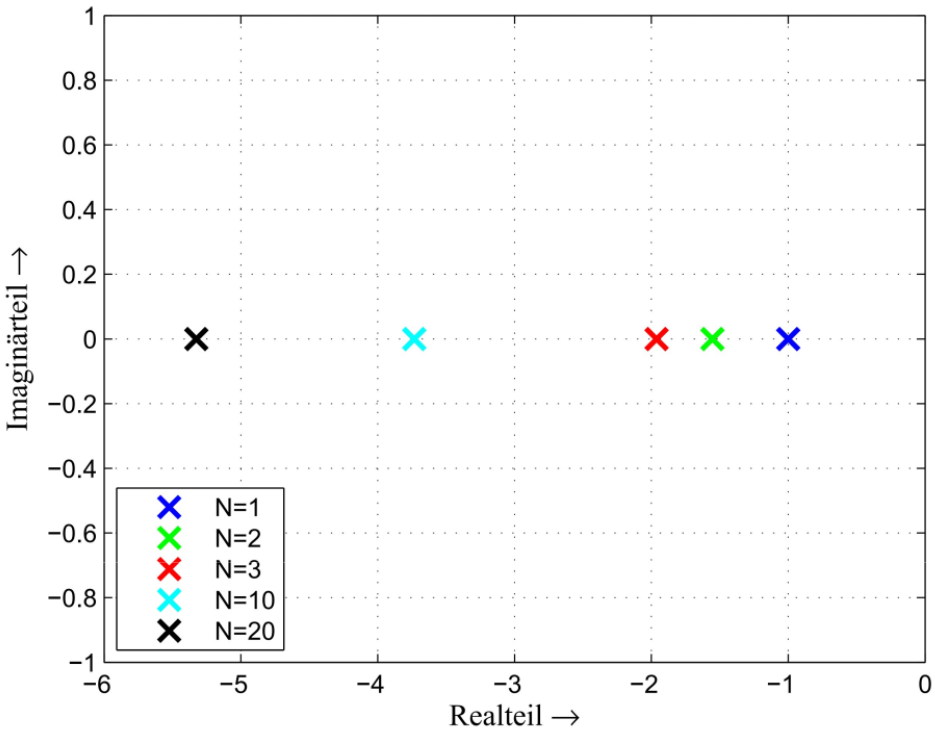
\includegraphics[width=\columnwidth]{images/filter_kritisch_gedaempft_pollagen.png}
\end{minipage}


\subsection{Approximation nach Butterworth}{303}

\begin{minipage}[c]{0.45\columnwidth}
    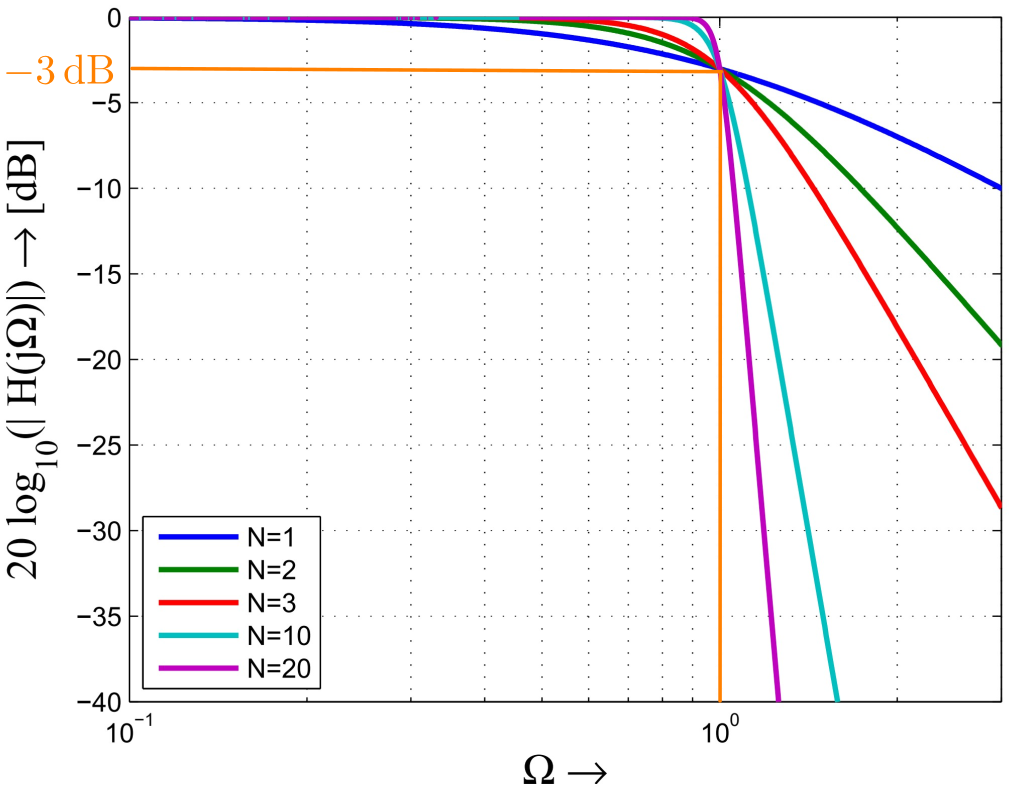
\includegraphics[width=\columnwidth]{images/filter_butterworth_amplitudengang.png}
\end{minipage}
\hfill
\begin{minipage}[c]{0.48\columnwidth}
    Die charakteristische Funktion wird bei der Butterworth-Approximation als\\
    $K(\Omega^2) = (\Omega^2)^n = \Omega^{2n}$ gewählt.

    Der Amplitudengang $|H(\jimg \Omega)|$ folgt somit der Gleichung

    $$\boxed{ |H(\jimg \Omega)| = \frac{1}{\sqrt{ 1 +\Omega^{2n}}} } $$
\end{minipage}


\subsubsection{Eigenschaften der Butterworth-Approximation}{303}

\begin{outline}
    \1 \textbf{Durchlassbereich}
        \2 Für $\Omega = 0$ ist für sämtliche $n$: $|H(0)| = H_{\rm max} = 1$
        \2 Für $\Omega = 1$ ist für sämtliche $n$: $|H(\jimg)| = \frac{H_{\rm max}}{\sqrt{2}} = \frac{1}{\sqrt{2}}$
            \textrightarrow\ $3 \, \deci \bel$ Dämpfung
        \2 Amplitudengang bei $\Omega = 0$ maximal flach, da alle Ableitungen $=0$ sind

    \1 \textbf{Sperrbereich}
        \2 Für $\Omega \gg 1$ wird $|H(\jimg \Omega)| \approx \frac{1}{\Omega^n}$ 
            \textrightarrow\ $\bm{- n \cdot 20 \, \deci \bel /}$ \textbf{Dekade}
    \1 \textbf{Allgemein}
        \2 Amplitudengang ist streng-monoton fallend \textrightarrow\ keine Welligkeit
\end{outline}


\subsubsection[Bestimmung von H(s) aus |H(jimg Omega)|]{Bestimmung von $H(s)$ aus $|H(\jimg \Omega)|$}{304}
\label{Bestimmung UTF aus Amplitudengang}

Aus dem Ansatz 
$$ | H(\jimg \Omega) |^2 = \frac{1}{1 + K(\Omega^2)} \Big|_{\Omega^2 = -S^2} = \frac{1}{1 + (-S^2)^n} = \cbl{H(S)} \cdot H(-S)
    = \cbl{\frac{1}{D(S)}} \cdot \frac{1}{D(-S)} $$
kann der folgende Teil isoliert betrachtet werden ($D(S)$ ist ein Hurwitz-Polynom):
$$ \boxed{ D(S) \cdot D(-S) = 1 + (-S^2)^n } $$

Mit dem Ansatz 
$$ \boxed{ D(S) = \prod\limits_{j=1}^{t} (S^2 + a_j \cdot S + b_j) \prod\limits_{j=2t+1}^{n} (S - c_j) } $$
wird das Produkt $D(S) \cdot D(-S)$ bestimmt. Anschliessend wird ein Koeffizientenvergleich durchgeführt.

\subsubsection{Bestimmung der Pol-Lage}{307}

Der Zusammenhang aus Abschnitt~\ref{Bestimmung UTF aus Amplitudengang} kann für die Bestimmung der Pole auf Null gesetzt werden:
$$ \boxed{ D(S) \cdot D(-S) = 1 + (-S^2)^n \overset{!}{=} 0 } $$
Durch Auflösen der Gleichung nach $S$ kommen die Pole auf dem \textbf{Einheitskreis} zu liegen.

\begin{itemize}
    \item Abstand zwischen den Polen: $\frac{\pi}{n}$
    \item Ordnung $n$ gerade: keine reellen Pole
    \item Ordnung $n$ ungerade: zwei reelle Pole bei $\pm 1$
    \item \textbf{Für Nennerpolynom $\bm{D(S) = \frac{1}{H(S)}}$ müssen nur Pole in der linken Halbebene berücksichtigt werden!}
\end{itemize}

\begin{center}
    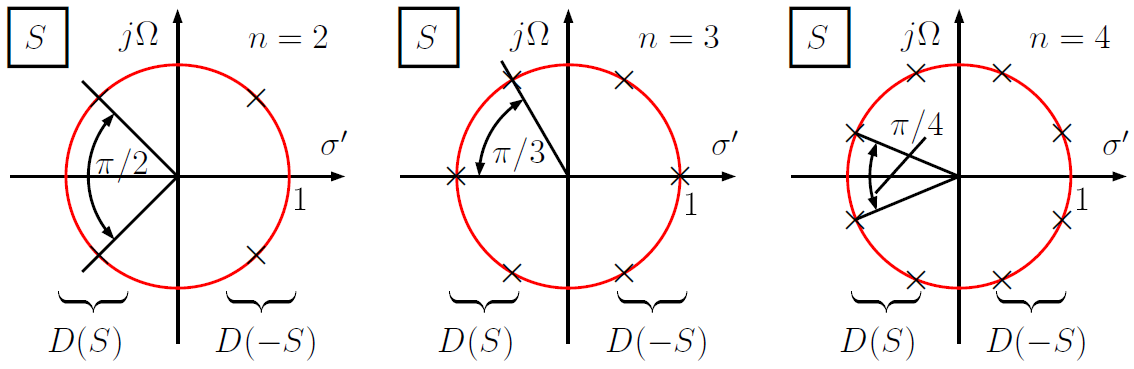
\includegraphics[width=0.8\columnwidth]{images/filter_pollage_butterworth.png}
\end{center}


\example{Butterworth 2. Ordnung -- $H(s)$ und Pol-Lage bestimmen}

$$ \text{Ansatz:} \quad H(S) \cdot H(-S) = \frac{1}{D(s)} \cdot \frac{1}{H(s)} = \frac{1}{ 1 + (-S^2)^n} $$

Für die Ordnung $n = 2$ ergibt sich das Nennerpolynom zu:
$$ D(S) \cdot D(-S) = 1 + S^4 \quad \Leftrightarrow \quad S^4 = -1 \quad \Leftrightarrow \quad
    e^{\jimg \bigl( \frac{\pi}{4} + k \frac{\pi}{2} \bigr)}$$

\begin{minipage}[c]{0.3\columnwidth}
    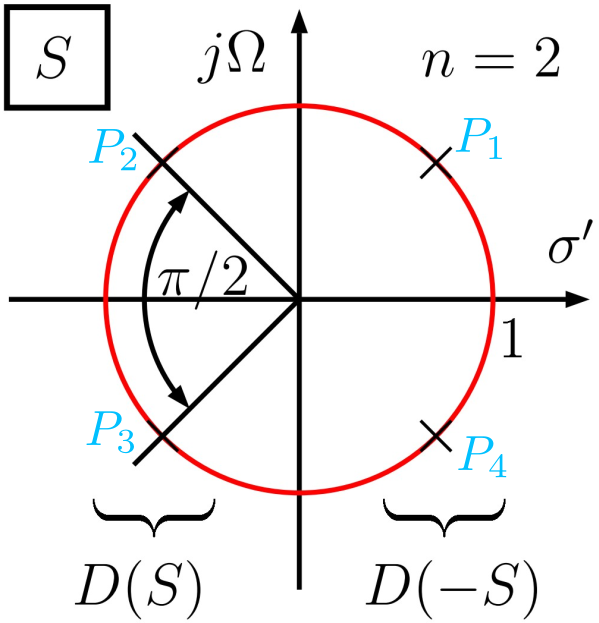
\includegraphics[width=\columnwidth]{images/filter_butterworth_pollagen_ordnung_2.png}
\end{minipage}
\hfill
\begin{minipage}[c]{0.58\columnwidth}
    Aufgelöst nach $S$ liegen die Nullstellen auf dem Einheitskreis mit Abstand $\frac{\pi}{4}$ verteilt.
    \vspace{0.2cm}

    \renewcommand{\arraystretch}{1.3}
    \begin{tabular}{c c}
        \textbf{Rechte Halbebene}                             & \textbf{Linke Halbebene} \\
        $P_1 = \frac{1}{\sqrt{2}} + \jimg \frac{1}{\sqrt{2}}$ & $P_2 = - \frac{1}{\sqrt{2}} + \jimg \frac{1}{\sqrt{2}}$ \\
        $P_4 = \frac{1}{\sqrt{2}} - \jimg \frac{1}{\sqrt{2}}$ & $P_3 = - \frac{1}{\sqrt{2}} - \jimg \frac{1}{\sqrt{2}}$ \\
    \end{tabular}
    \renewcommand{\arraystretch}{1}

    \vspace{0.2cm}
    \textrightarrow Für die Übertragungsfunktion $H(s)$ sind nur die Nullstellen in der \textbf{linken Halbebene} relevant!
\end{minipage}

\vspace{0.2cm}
Die Übertragungsfunktion $H(s)$ ergibt sich aus
$$ H(s) = \frac{1}{D(s)} = \frac{1}{(S - P_2) \cdot (S - P_3)} = \frac{1}{S^2 + \sqrt{2} S + 1} $$


Alternativ kann die Übertragungsfunktion $H(S)$ auch mittels folgendem Ansatz für $D(S)$ und anschliessendem Koeffizientenvergleich
von $D(S) \cdot D(-S)$ bestimmt werden.

$$ \text{Ansatz:} \quad  D(S) =  S^2 + a_1 S + b_1 $$
$$ \text{Koeffizientenvergleich:} \quad D(S) \cdot D(-S) = S^4 + (2 b_1 - a_1^2) \, S + b_1^2 \overset{!}{=} S^4 + 1 $$
\textrightarrow\ $a_1 = \sqrt{2}$ und $b_1 = 1$ \quad \textrightarrow\ $S^2 + \sqrt{2} S + 1$ 
\quad \textrightarrow\ $H(s) = \frac{1}{D(s)} = \frac{1}{S^2 + \sqrt{2} S + 1}$


\subsubsection{Bestimmung der Filterordnung}{308}

Aus dem Toleranzschema lassen sich für die 'Ecken' die folgenden beiden Bedingungen aufstellen:

\begin{minipage}[c]{0.48\columnwidth}
    $$ A(\Omega_D) = 10 \cdot \log_{10}(1 + \Omega_D^{2n}) = A_{\rm max} $$
\end{minipage}
\hfill
\begin{minipage}[c]{0.48\columnwidth}
    $$ A(\Omega_S) = 10 \cdot \log_{10}(1 + \Omega_S^{2n}) = A_{\rm min} $$
\end{minipage}

\vspace{0.2cm}
\begin{minipage}[c]{0.48\columnwidth}
    Mittels Umformungen und aufgelöst nach $n$ ergibt sich die Filter-Ordnung als \\
    $\left\lceil . \right\rceil $ bedeutet '\textbf{aufrunden} auf ganze Zahl'
\end{minipage}
\hfill
\begin{minipage}[c]{0.48\columnwidth}
    $$ \boxed{ n =  \left\lceil \frac{\log_{10} \Bigl( \frac{10^{A_{\rm min / 10}} - 1}{10^{A_{\rm max / 10}} - 1}  \Bigr) }
        {2 \cdot \log_{10}\Bigl( \frac{\Omega_S}{\Omega_D} \Bigr)}  \right\rceil } $$
\end{minipage}

\textrightarrow\ Alternativ kann die Ordnung $n$ auch mit dem Nomogramm bestimmt werden.

% --------------------------------------------------------------------------------------------------
\subsection{Approximation nach Tschebyscheff-\uproman{1}}{310}

\begin{minipage}[c]{0.45\columnwidth}
    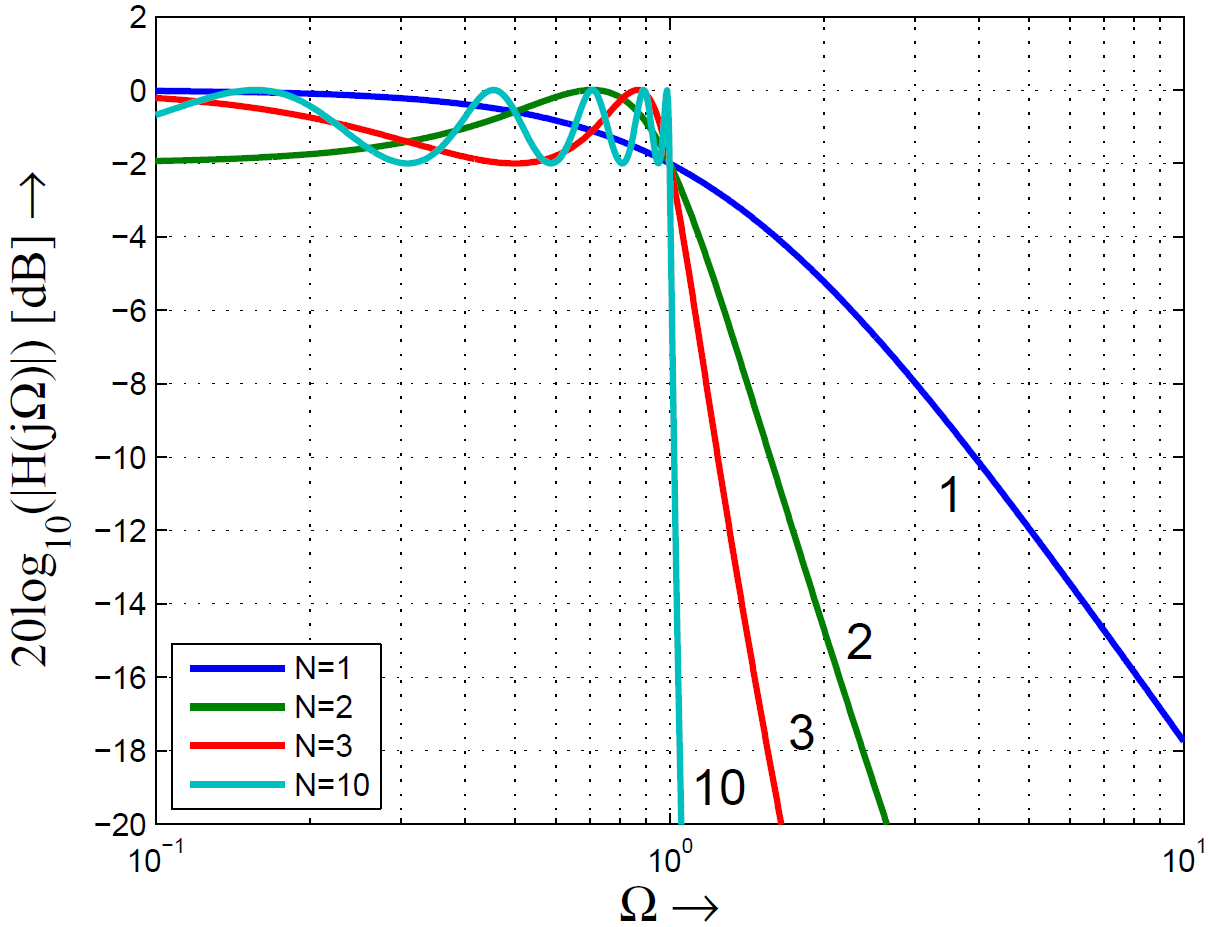
\includegraphics[width=\columnwidth]{images/filter_tschebyscheff_amplitudengang.png}
\end{minipage}
\hfill
\begin{minipage}[c]{0.48\columnwidth}
    Die charakteristische Funktion wird bei der Tschebyscheff-\uproman{1} als\\
    $K(\Omega^2) = e^2 \cdot C_n^2(\Omega)$ gewählt.

    Der Amplitudengang $|H(\jimg \Omega)|$ folgt somit der Gleichung

    $$\boxed{ |H(\jimg \Omega)| = \frac{1}{\sqrt{1 + e^2 \cdot C_n^2(\Omega)} } } $$

    \begin{tabular}{ll@{}}
        $e$             & \textbf{Rippelfaktor} (Konstante) \\
        $C_n(\Omega)$   & Tschebyscheff-Polynom erster\\
                        & Art der Ornung $n$
    \end{tabular}
\end{minipage}

Das Tschebyscheff-Polynom $C_n(\Omega)$ ist im Durchlassbereich und im Sperrbereich \textbf{unterschiedlich definiert!}

\vspace{0.2cm}

\begin{minipage}[c]{0.48\columnwidth}
    \begin{center}
        \myul{Duchlassbereich $(|\Omega| \leq 1)$}
        $$ \boxed{ C_n(\Omega) = \cos(n \cdot \arccos(\Omega)) } $$
    \end{center}
    
\end{minipage}
\hfill
\begin{minipage}[c]{0.48\columnwidth}
    \begin{center}
        \myul{Sperrbereich $(|\Omega| \geq 1)$}
        $$ \boxed{ C_n(\Omega) = \cosh(n \cdot \mathrm{arccosh}(\Omega)) } $$
    \end{center}
\end{minipage}

\vspace{0.2cm}
Für die Ordnung $n \geq 2$ lässt sich das Tschebyscheff-Polynom $C_n(\Omega)$ mittels Rekursionsformel berechnen
$$ \boxed{ C_n(\Omega) = 2 \, \Omega \, C_{n-1}(\Omega) - C_{n-2}(\Omega) }  \qquad C_0(\Omega) = 1 \qquad C_1(\Omega) = \Omega $$

Zwischen dem Rippelfaktor $e$ und der maximalen Dämpfung $A_{\rm max}$ gilt der Zusammenhang:
$$ \boxed{ A_{\rm max} = 10 \cdot \log_{10}(1 + e^2) \quad \Leftrightarrow \quad e = \sqrt{10^{\frac{A_{\rm max}}{10}} -1} } $$


\subsubsection{Eigenschaften der Tschebyscheff-\uproman{1}-Approximation}{311}

Im \textbf{Durchlassbereich} schwankt das Tschebyscheff-Polynom in den Grenzen $\pm 1$. Im \textbf{Sperrbereich} nimmt
$C_n$ monoton mit $\Omega$ zu.

\begin{center}
    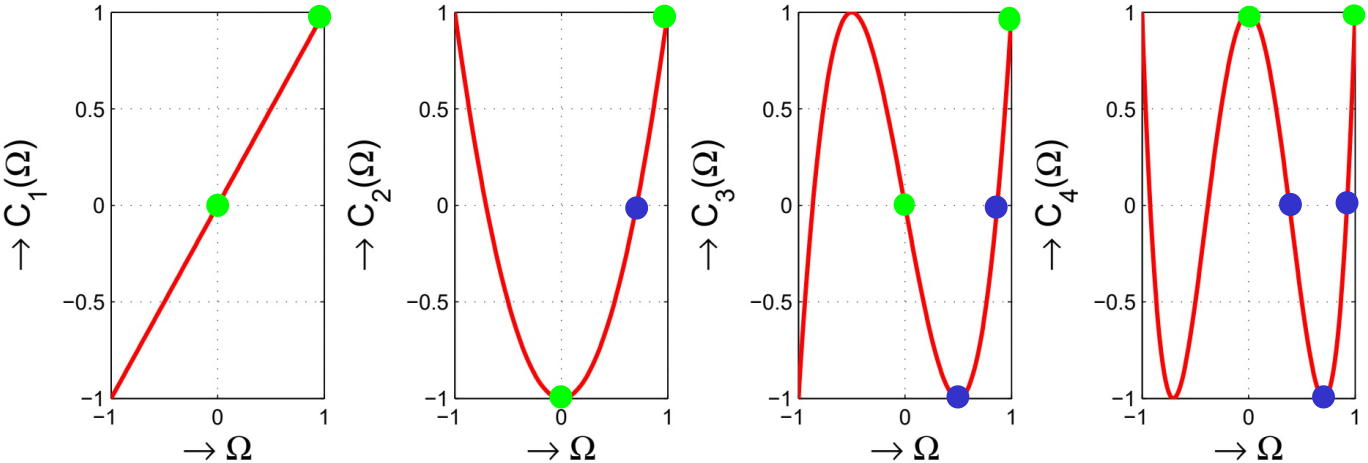
\includegraphics[width=0.8\columnwidth]{images/filter_tschebyscheff_ordnung_ablesen.png}
\end{center}


\begin{outline}
    \1 \textbf{Durchlassbereich}
        \2 Für $\Omega = 0$ ist für \textbf{un}gerade $n$: $|H(0)| = H_{\rm max} = 1$
        \2 Für $\Omega = 0$ ist für gerade $n$: $|H(0)| = \frac{1}{\sqrt{1 + e^2}}$
        \2 Für $\Omega = 1$ ist für sämtliche $n$: $|H(\jimg)| = \frac{1}{\sqrt{1 + e^2}}$ 
            \textrightarrow\ \textbf{nicht} $3 \, \deci \bel$ Dämpfung
        \2 Aus der Anzahl \textbf{\cbl{Extremalstellen} und \cgn{Endpunkte}} des Amplitudengangs im \textbf{Durchlassbereich} 
            $(0 \leq \Omega \leq 1)$ lässt sich die \textbf{Ordnung $\bm{n}$} bestimmen. \\
            \textbf{Ordnung = Summe aller \cbl{Extremalstellen} plus beide  \cgn{Endpunkte} minus 1}
    \1 \textbf{Sperrbereich}
        \2 Für $\Omega \gg 1$ wird $|H(\jimg \Omega)| \approx \frac{1}{e \cdot C_n(\Omega)}$ 
            \textrightarrow\ $\bm{- n \cdot 20 \, \deci \bel /}$ \textbf{Dekade} bzw.\\
            $\bm{- n \cdot 6.02 \, \deci \bel /}$ \textbf{Oktave}
        \2 Fixe Ordnung $n$: Je grösser der Rippelfaktor $e$, desto steiler der Abfall in den Sperrbereich
        \2 Fixer Rippelfaktor $e$: Je grösser die Ordnung $n$, desto steiler der Abfall in den Sperrbereich
\end{outline}


\begin{minipage}[t]{0.48\columnwidth}
    \subsubsection{Pol-Lagen}{313}

    \begin{itemize}
        \item Die Pole liegen auf einer \textbf{Ellipse}
        \item Allpolfilter
        \item Je näher die Pole an der $\jimg \omega$-Achse liegen, desto mehr Rippel gibt es im Phasengang %CHECK: Phasengang oder Amplitudengang?
    \end{itemize}
\end{minipage}
\hfill
\begin{minipage}[t]{0.48\columnwidth}
    \subsubsection{Filterordnung}{316}

    $$ \boxed{ n =  \left\lceil \frac{\arccos \Bigl( \sqrt{ \frac{10^{A_{\rm min / 10}} - 1}{10^{A_{\rm max / 10}} - 1} } \Bigr) }
        {\arccos \Bigl( \frac{\Omega_S}{\Omega_D} \Bigr)}  \right\rceil } $$
    \textrightarrow\ Nomgramme!
\end{minipage}


\subsection{Approximation nach Tschebyscheff-\uproman{2}}{319}

\begin{minipage}[c]{0.45\columnwidth}
    \textbf{Inverses Tschebyscheff-Filter}

    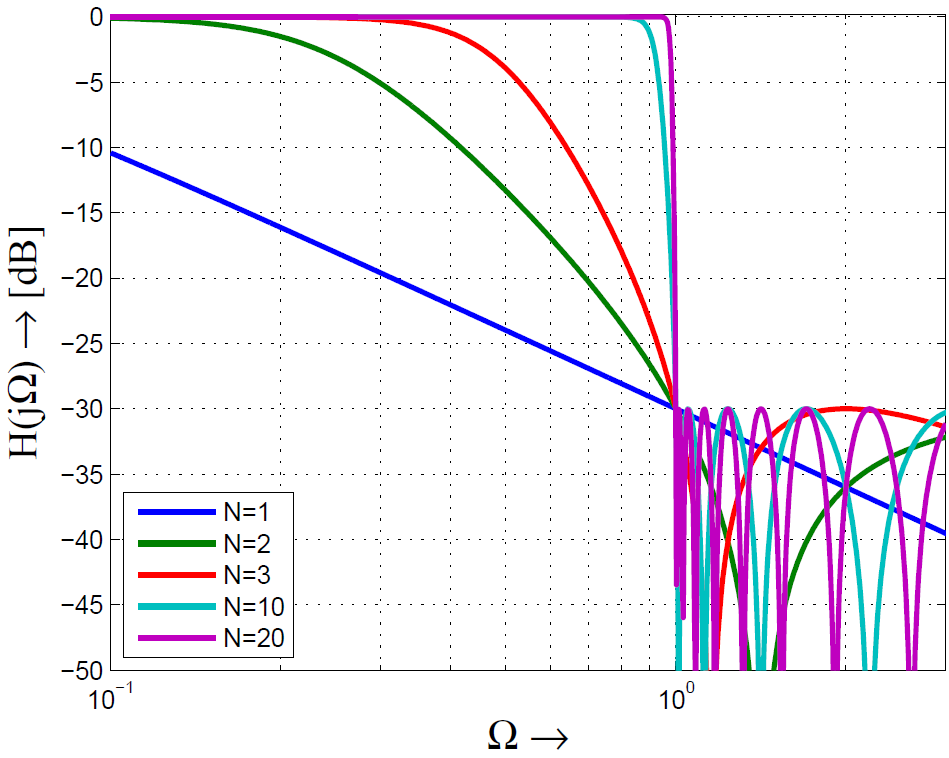
\includegraphics[width=\columnwidth]{images/filter_tschebyscheff_invers_amplitudengang.png}
\end{minipage}
\hfill
\begin{minipage}[c]{0.48\columnwidth}
    Die charakteristische Funktion wird bei der Tschebyscheff-\uproman{2}-Approximation als\\
    $K(\Omega^2) = e^2 \cdot C_n^2(\Omega)$ gewählt.

    Der Amplitudengang $|H(\jimg \Omega)|$ folgt somit der Gleichung

    $$ \boxed{ |H(\jimg \Omega)| = \frac{1}{\sqrt{1 + \frac{1}{e^2 C_n^2  \big(\frac{1}{\Omega} \big) }}} } $$

    \begin{tabular}{ll@{}}
        $e$             & \textbf{Rippelfaktor} (Konstante) \\
        $C_n(\Omega)$   & Tschebyscheff-Polynom erster\\
                        & Art der Ornung $n$
    \end{tabular}
\end{minipage}


\subsubsection{Pol-Lagen}{321}

\begin{minipage}[c]{0.4\columnwidth}
    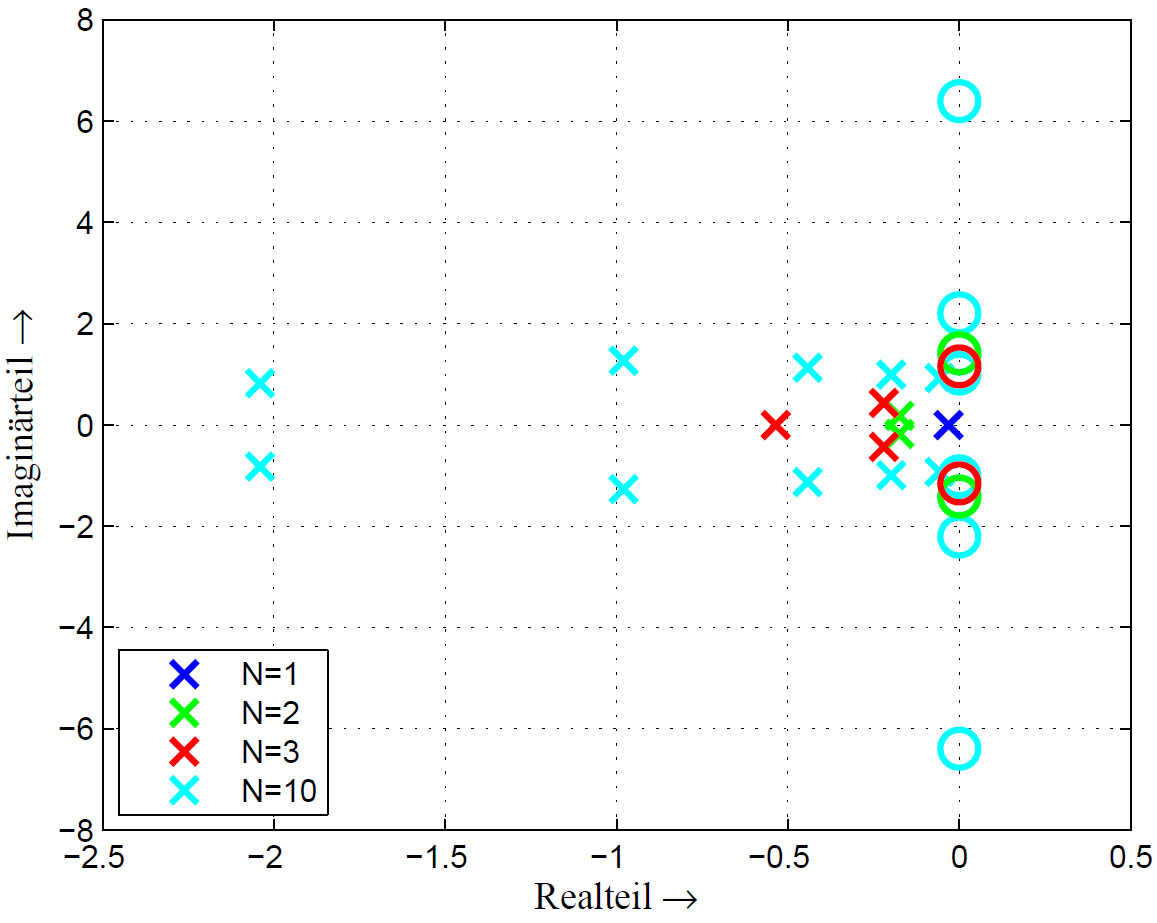
\includegraphics[width=\columnwidth]{images/filter_tschebyscheff_invers_pollage.png}
\end{minipage}
\hfill
\begin{minipage}[c]{0.58\columnwidth}
    \begin{outline}
        \1 \textbf{Kein} Allpolfilter
            \2 Gerade Ordnung $n$: $n$ Pole und $n$ Nullstellen
            \2 \textbf{Un}gerade Ordnung $n$: $n$ Pole und $n-1$ Nullstellen
    \end{outline}
\end{minipage}


\subsubsection{Filterordnung}{319}

\begin{minipage}[c]{0.4\columnwidth}
    $$ \boxed{ n =  \left\lceil \frac{\arccos \Bigl( \sqrt{ \frac{10^{A_{\rm min / 10}} - 1}{10^{A_{\rm max / 10}} - 1} } \Bigr) }
    {\arccos \Bigl( \frac{\Omega_S}{\Omega_D} \Bigr)}  \right\rceil } $$
\end{minipage}
\hfill
\begin{minipage}[c]{0.58\columnwidth}
    Die Filterordnung berechnet sich identisch wie bei der Tschebyscheff-\uproman{1}-Approximation! \\
    \textrightarrow\ Gleiches Nomogramm wie für Tschebyscheff-\uproman{1}
\end{minipage}


\subsection{Approximation nach Cauer}{322}

\begin{minipage}[c]{0.45\columnwidth}
    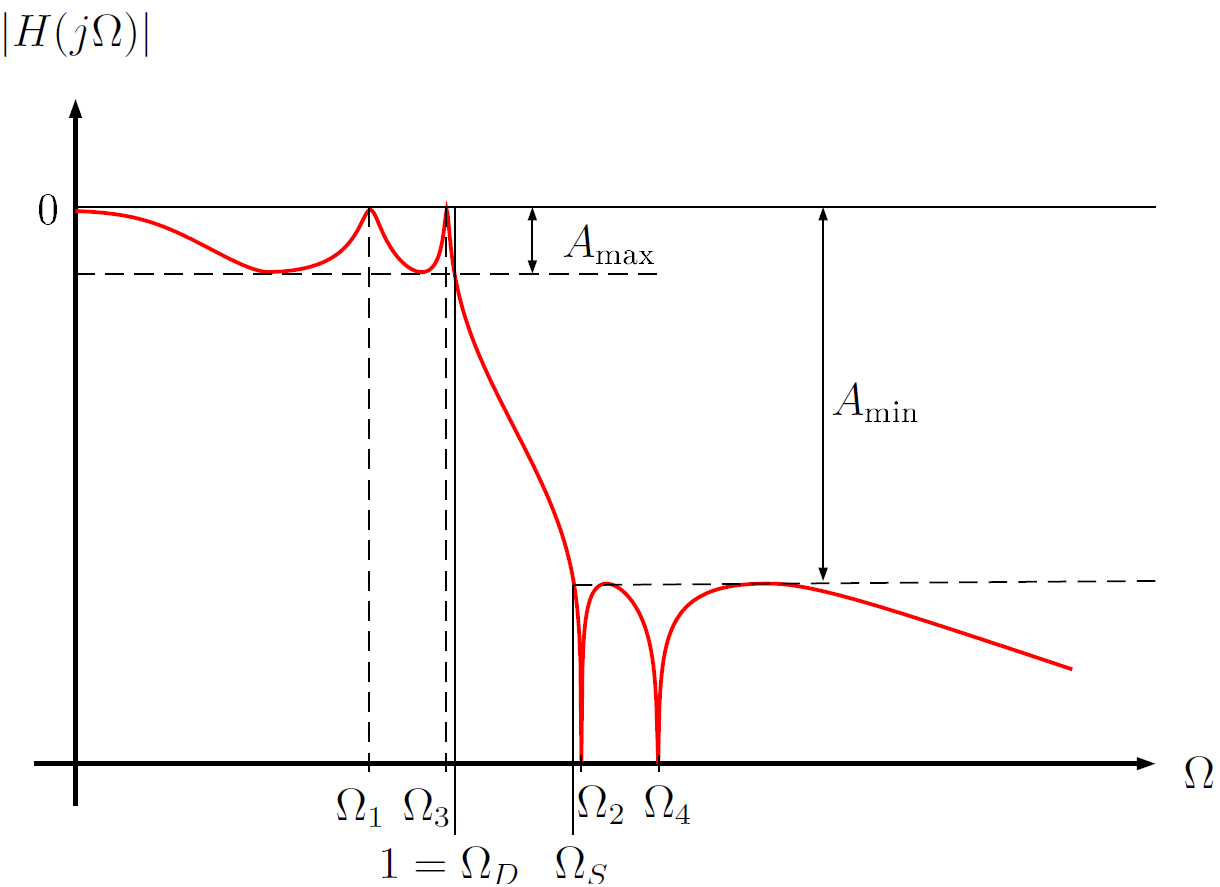
\includegraphics[width=\columnwidth]{images/filter_cauer_amplitudengang.png}
\end{minipage}
\hfill
\begin{minipage}[c]{0.48\columnwidth}
    \textbf{Kombination von Tschebyscheff-\uproman{1} und Tschebyscheff-\uproman{2}} \\

    Daher spricht man auch von Complete-Chebyshev- oder Chebyshev-Cauer-Filtern (CC-Filter).
\end{minipage}


\subsubsection{Pol-Lagen}{325}

\begin{minipage}[c]{0.4\columnwidth}
    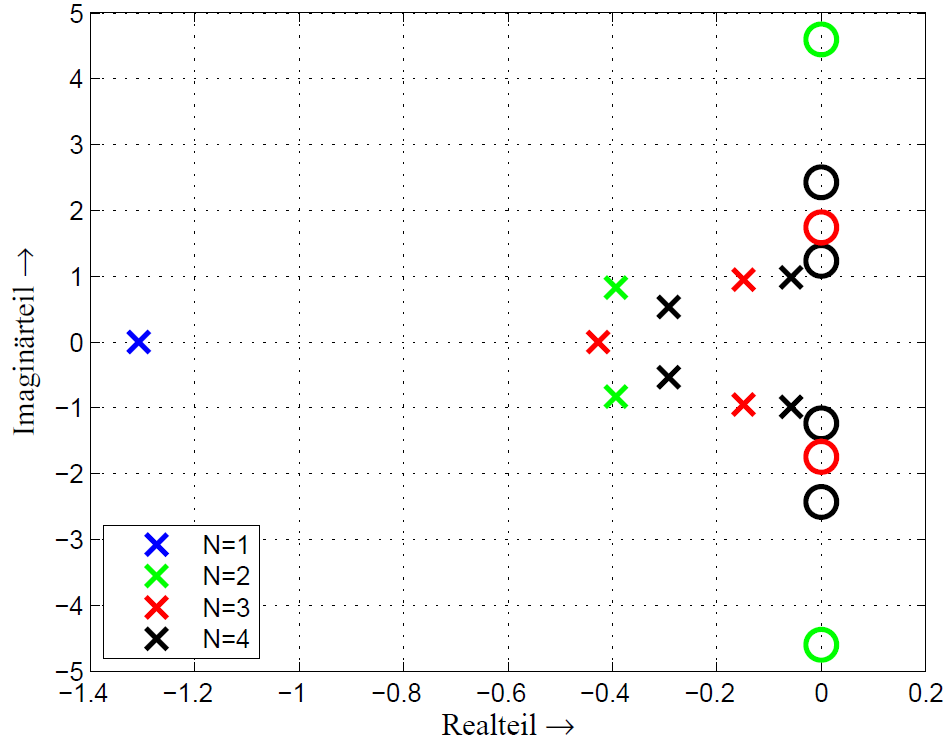
\includegraphics[width=\columnwidth]{images/filter_cauer_pollage.png}
\end{minipage}
\hfill
\begin{minipage}[c]{0.58\columnwidth}
    \begin{outline}
        \1 \textbf{Kein} Allpolfilter
            \2 Gerade Ordnung $n$: $n$ Pole und $n$ Nullstellen
            \2 \textbf{Un}gerade Ordnung $n$: $n$ Pole und $n-1$ Nullstellen
    \end{outline}
\end{minipage}


\subsubsection{Filterordnung}{326}

$$ \boxed{ n = \left\lceil \frac{ K \Bigg( \Big( \frac{\Omega_D}{\Omega_S} \Big)^2 \Bigg) \, K \Bigg( 1 - \frac{A_{\rm max / 10} - 1}{A_{\rm min / 10} - 1} \Bigg) }
    { K \Bigg( 1 -\Big( \frac{\Omega_D}{\Omega_S} \Big)^2 \Bigg) \, K \Bigg(\frac{A_{\rm max / 10} - 1}{A_{\rm min / 10} - 1} \Bigg) }  \right\rceil 
    \quad \text{mit } K(k) = \int\limits_{0}^{\frac{\pi}{2} }  \frac{1}{\sqrt{1- k \sin^2(\theta)}} \, \diff \theta }$$
    \textrightarrow\ Nomogramm!


\subsection{Approximation nach Bessel}{328}

\begin{minipage}[c]{0.45\columnwidth}
    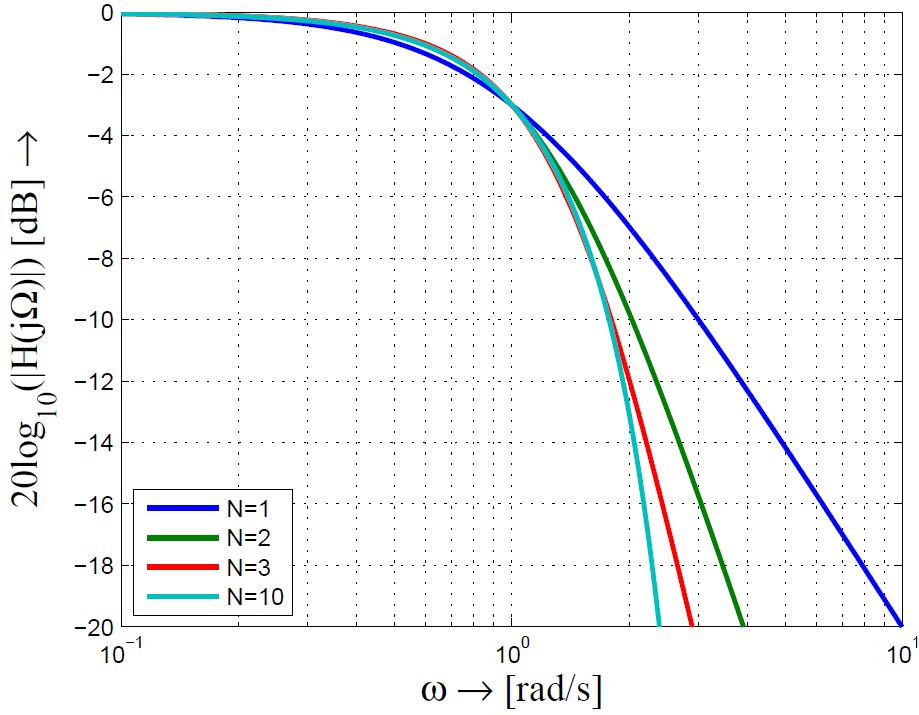
\includegraphics[width=\columnwidth]{images/filter_bessel_amplitudengang.png}
\end{minipage}
\hfill
\begin{minipage}[c]{0.48\columnwidth}
    Bessel-Filter liefern eine möglichst \textbf{lineare Phase}, d.h. eine \textbf{konstante Gruppenlaufzeit}.

    Die Übertragungsfunktion $H(S)$ lautet
    $$ \boxed{ H(S) = K \cdot e^{-S T_0} } $$

    Für die Gruppenlaufzeit folgt somit
    $$ \boxed{ \tau_g(\Omega) = \frac{- \diff \theta(\Omega)}{\diff \Omega} = T_0 = \const } $$
\end{minipage}

\vspace{0.2cm}
Ohne Einschränkung kann in der UTF $T_0 = 1$ und $K = 1$ gesetzt werden:
$$ H(S) = e^{-S} = \frac{1}{e^S} \approx \frac{1}{D(S)} $$


\subsubsection{Gruppenlaufzeit $\tau_g(\Omega)$ und Phasenlaufzeit $\tau_p(\Omega)$}{331}

\begin{minipage}[c]{0.4\columnwidth}
    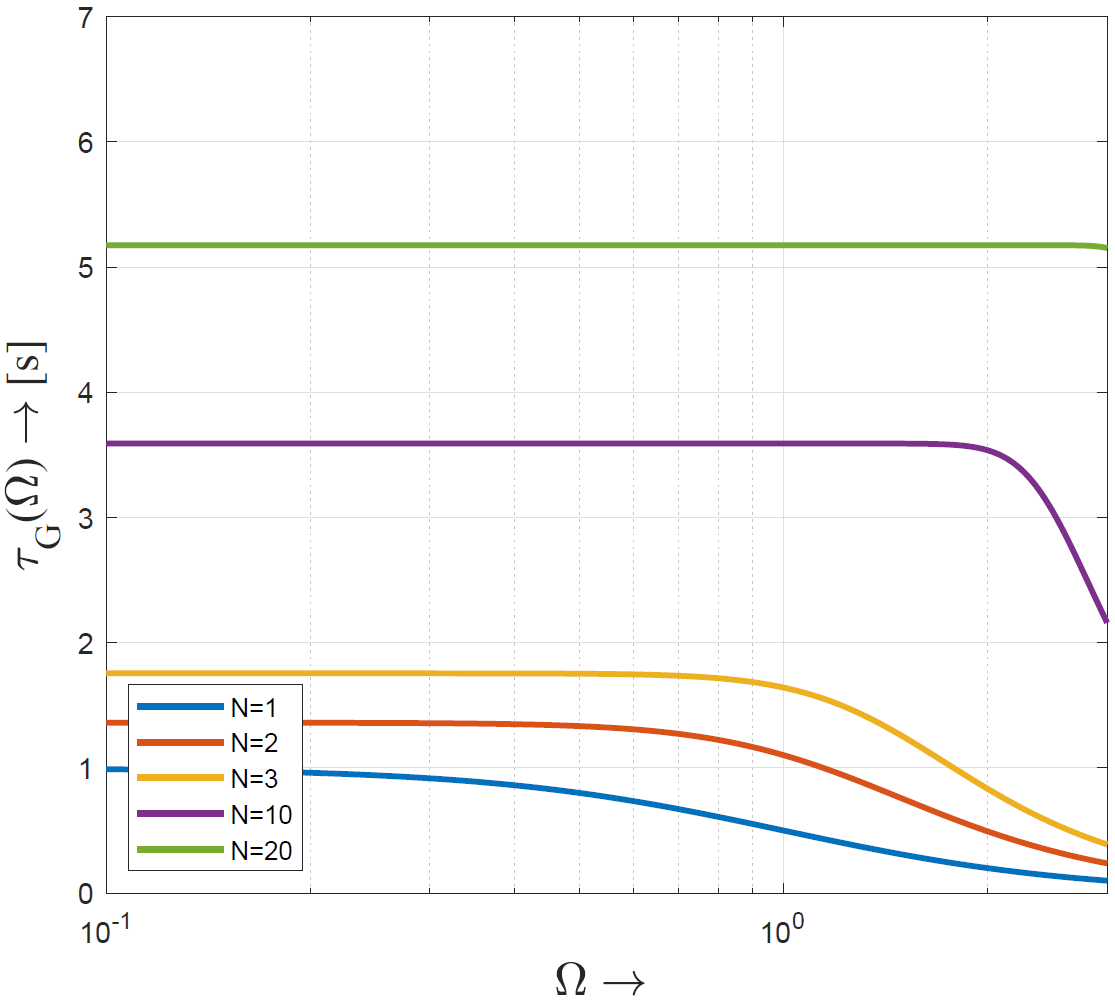
\includegraphics[width=\columnwidth]{images/filter_bessel_gruppenlaufzeit.png}
\end{minipage}
\hfill
\begin{minipage}[c]{0.4\columnwidth}
    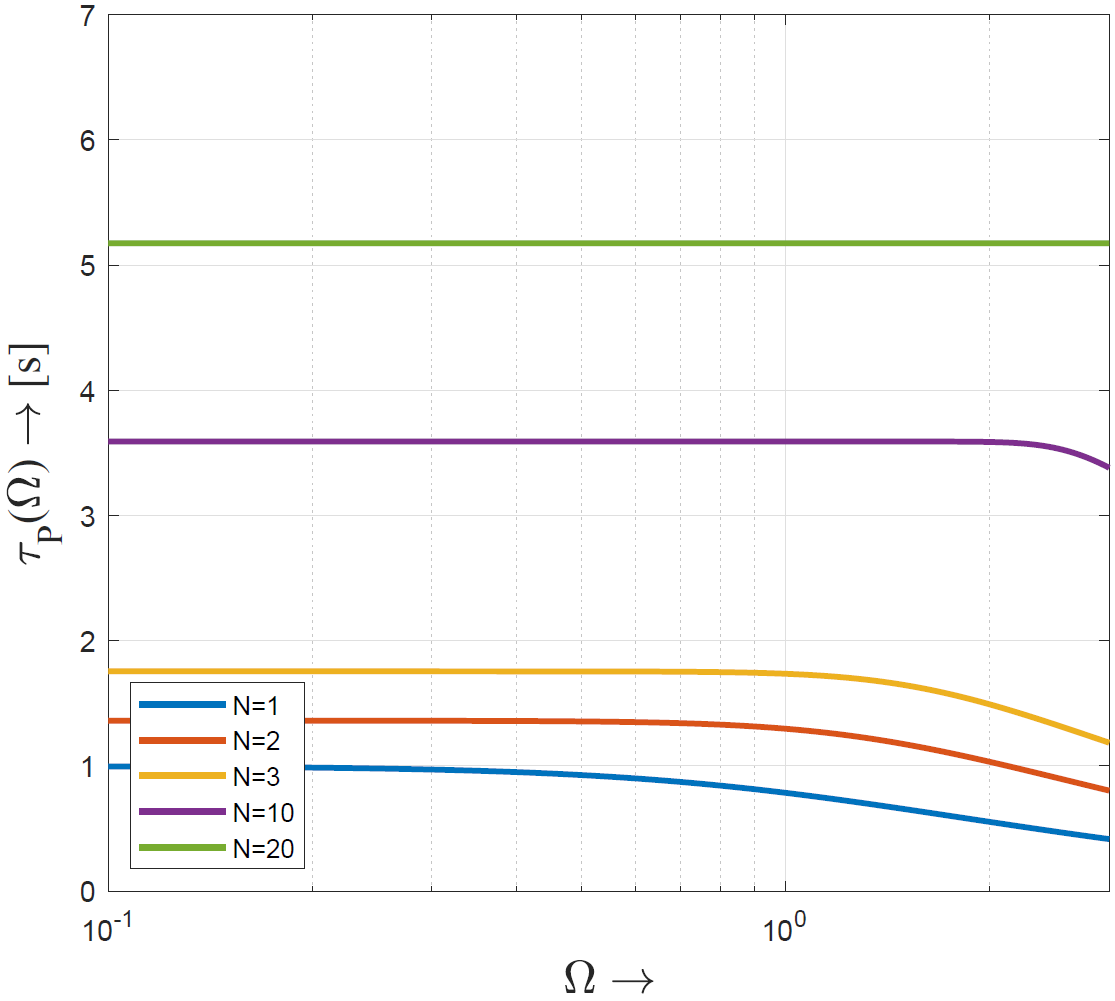
\includegraphics[width=\columnwidth]{images/filter_bessel_phasenlaufzeit.png}
\end{minipage}


\subsection{Gegenüberstellung der Filter-Approximationen}

\scalebox{0.68}{
\begin{tabular}{|l|c|c|c|c|c|c|}
    \hline
    \multicolumn{1}{|c|}{} & \textbf{Krit. Gedämpft}                                            & \textbf{Butterworth}                                                    & \textbf{Tschebyscheff 1}                                        & \textbf{Tschebyscheff 2}                                       & \textbf{Cauer}       & \textbf{Bessel}                                          \\ \hline
    \textbf{Allpolfilter}  & ja                                                                 & ja                                                                      & ja                                                              & nein                                                           & nein                 & ja                                                       \\ \hline
    \textbf{Pol-Lage}      & \begin{tabular}[c]{@{}c@{}}reelle Achse\\ \textless 0\end{tabular} & \begin{tabular}[c]{@{}c@{}}Halbkreis\\ LHE\end{tabular}                 & \begin{tabular}[c]{@{}c@{}}Ellipse\\ LHE\end{tabular}           & LHE                                                            & LHE                  & \begin{tabular}[c]{@{}c@{}}exzentr.\\ Kreis\end{tabular} \\ \hline
    \textbf{NS-Lage}       & -                                                                  & -                                                                       & -                                                               & $\jimg \omega$-Achse                                           & $\jimg \omega$-Achse & -                                                        \\ \hline
    \textbf{DB}            & streng monoton                                                     & \begin{tabular}[c]{@{}c@{}}streng monoton\\ steilstmöglich\end{tabular} & \begin{tabular}[c]{@{}c@{}}wellig\\ konst. Rippel\end{tabular}  & streng monoton                                                 & wellig               & streng monoton                                           \\ \hline
    \textbf{SB}            & streng monoton                                                     & streng monoton                                                          & streng monoton                                                  & \begin{tabular}[c]{@{}c@{}}wellig\\ konst. Rippel\end{tabular} & wellig               & streng monoton                                           \\ \hline
    \textbf{Phasengang}    & sehr gut                                                           & mittel                                                                  & schlecht                                                        & schlecht                                                       & wild                 & bestmöglich                                              \\ \hline
\end{tabular}}


\subsubsection{Frequenzgänge / Lage der Pol- und Nullstellen}{334}

\begin{minipage}[c]{0.7\columnwidth}
    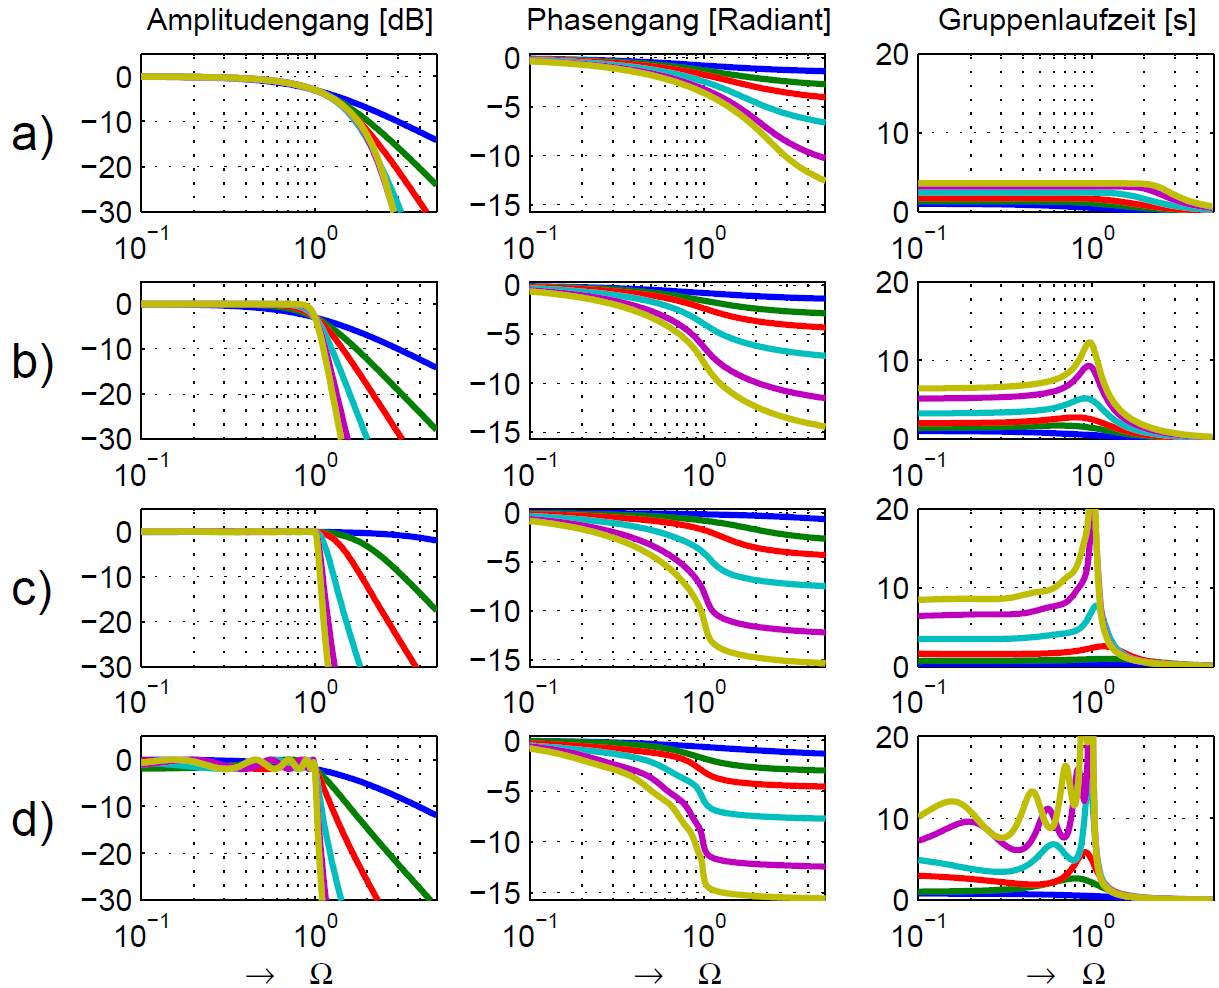
\includegraphics[width=\columnwidth]{images/filter_vergleich_frequenzgaenge.png}
\end{minipage}
\hfill
\begin{minipage}[c]{0.28\columnwidth}
    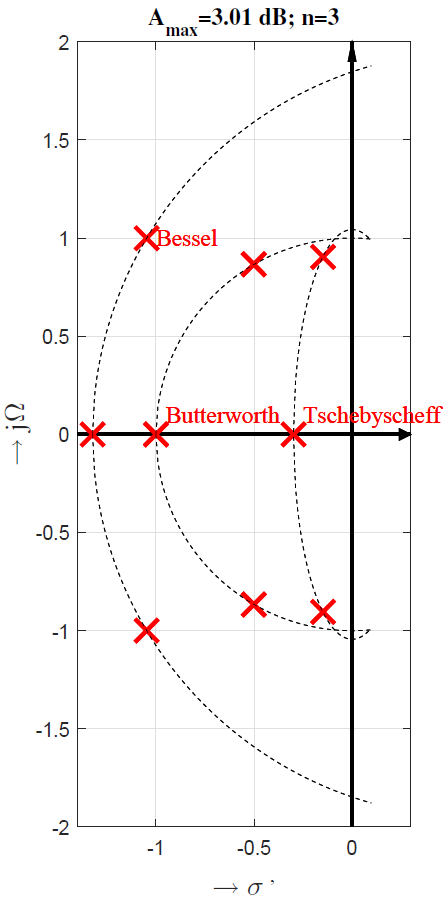
\includegraphics[width=\columnwidth]{images/filter_vergleich_pollagen.png}
\end{minipage}

\begin{tabular}{ll cc ll}
    a) & Bessel         & & & c) & Tschebyscheff ($0.1 \, \deci \bel$) \\
    b) & Butterworth    & & & d) & Tschebyscheff ($2 \, \deci \bel$) \\
\end{tabular}


% ----------------------------------------------------------------------------------------------------------------
% ev. in einege section bzw eigenes file für "oberflächliches zeugs" packen
% deep dive (von oben) dann auch in eigene section

% CHECK: Wohin mit dieser subsection?
\subsection{Standard-Filtertypen -- Überblick}
\label{Standard-Filtertypen}

\begin{outline}
    % TODO: Symbol für 2. Ebene lokal bzw. hier explizit ändern? auf was?
    \1 \textbf{kritisch-Gedämpfte Filter}
        \2[+] \textbf{Kein Rippel} im Durchlass- und Sperrbereich
        \2[+] Kein Überschwingen bei Impuls- und Sprungantwort
        \2[-] Braucht \textbf{hohe Ordnung} für steilen Übergang von Durchlass- zu Sperrbereich
        \2    Kaskadierung von $n$ wirkungsfreien, identischen Filtern 1. Ordnung
        \2    Bei $\Omega = 1$ \textrightarrow\ Dämpfung von $3 \, \deci \bel$
        \2    Steilheit: $- n \cdot 20 \, \deci \bel /$ Dekade
        \2    Allpolfiler: $n$ Pole am gleichen Ort in der LHE

    \1 \textbf{Butterworth}
        \2[+] \textbf{Kein Rippel} im Durchlass- und Sperrbereich
        \2[+] Im Durchlassbereich ist der Amplitudengang \textbf{maximal flach}
        \2[-] Überhöhung in der Gruppenlaufzeit der Grenzfrequenz
        \2[-] Braucht \textbf{hohe Ordnung} für steilen Übergang von Durchlass- zu Sperrbereich
        \2    Bei $\Omega = 1$ \textrightarrow\ Dämpfung von $3 \, \deci \bel$
        \2    Steilheit: $- n \cdot 20 \, \deci \bel /$ Dekade
        \2    Allpolfiler: Pole auf Einheitskreis mit Abstand $\frac{\pi}{n}$ 

    \1 \textbf{Tschebyscheff-\uproman{1}}
        \2[+] Schon für kleine Ordnungen \textbf{relativ steil} im Übergang von Durchlass- und Sperrbereich
        \2[-] \textbf{Rippel} im \textbf{Durchlassbereich} (abhängig von Ordnung $n$)
        \2[-] Keine konstante Gruppenlaufzeit (wellig)
        \2    Bei $\Omega = 1$ \textrightarrow\ Dämpfung abhängig von Rippelfaktor $e$
        \2    Steilheit: $- n \cdot 20 \, \deci \bel /$ Dekade
        \2    Allpolfiler: Pole auf einer Ellipse

    \1 \textbf{Tschebyscheff-\uproman{2}}
        \2[+] Schon für kleine Ordnungen \textbf{relativ steil} im Übergang von Durchlass- und Sperrbereich
        \2[-] \textbf{Rippel} im \textbf{Sperrbereich} (abhängig von Ordnung $n$)
        \2[-] Relativ konstante Gruppenlaufzeit
        \2    Bei $\Omega = 1$ \textrightarrow\ Dämpfung abhängig von Rippelfaktor $e$
        \2    Steilheit: $- n \cdot 20 \, \deci \bel /$ Dekade
        \2    Kein Allpolfilter

    \1 \textbf{Cauer}
        \2[+] Steilster Übergang von Durchlass- zu Sperrbereich
        \2[-] \textbf{Rippel} in \textbf{Durlassbereich und Sperrbereich} (abhängig von Ordnung $n$)
        \2    \textbf{Kombination aus Tschebyscheff-\uproman{1} und Tschebyscheff-\uproman{2}}
        % \2    Steilheit: $- n \cdot 20 \, \deci \bel /$ Dekade
        \2    Kein Allpolfilter

    \1 \textbf{Bessel}
        \2[+] \textbf{Flachster Übergang} von Durchlass- und Sperrbereich von allen Filtern
        \2[+] Konstante Gruppenlaufzeit
        \2[-] Für steile Filter im Durchlass- und Sperrbereich nicht geeignet
        \2    Allpolfilter: Pole auf exzentrischen Kreisen in LHE
\end{outline}


% CHECK: Wohin mit dieser Subsection?
% TODO: verbessern
\subsection{Vorgehen Filter dimensionieren / auslegen}

\begin{enumerate}
    \item Gemäss Anforderungen geeigneten Filtertyp wählen (\textrightarrow\ \ref{Standard-Filtertypen})
    \item Toleranzschema gemäss Anforderungen erstellen inkl. Normierung (\textrightarrow\ \ref{Toleranzschema})
    \item Ordnung des Filters bestimmen (Formel oder Nomogramm \textrightarrow\ \ref{Nomogramme})
    \item Übertragungsfunktion bestimmen (\textrightarrow\ Tabellen oder Matlab)
    \item Komponenten mittels Entnormierung bestimmen (Tabellen \textrightarrow\ \ref{Tabellen})
\end{enumerate}


% CHECK: Wohin mit dieser Subsection?
\subsection{Nomogramme}{393}
\label{Nomogramme}

Nomogramme können verwendet werden, um die \textbf{Ordnung eines Filters}  zu bestimmen.

\begin{minipage}[c]{0.42\columnwidth}
    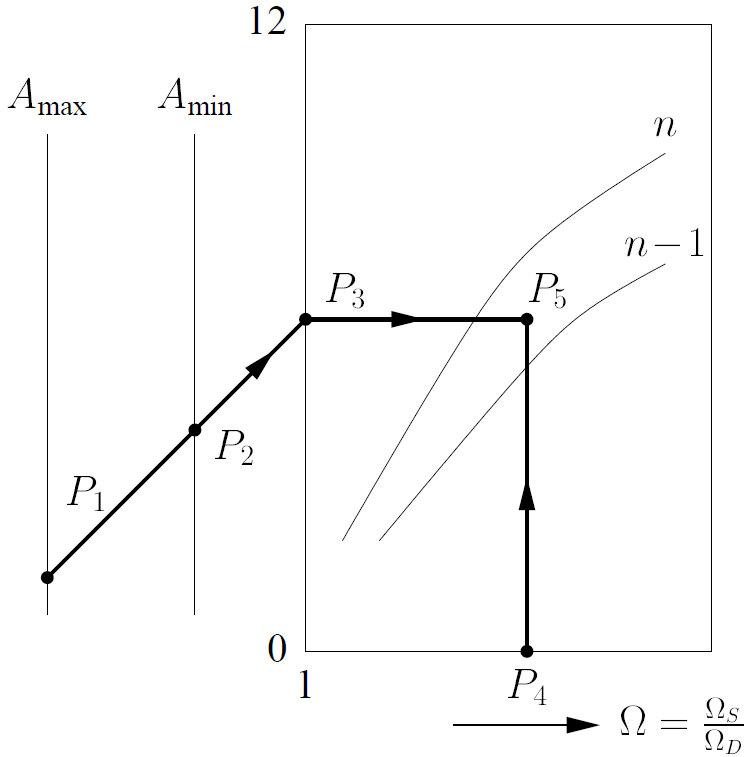
\includegraphics[width=\columnwidth]{images/filter_nomogramme.png}
\end{minipage}
\hfill
\begin{minipage}[c]{0.56\columnwidth}
    \begin{center}
        \textbf{\myul{Benutzung von Nomogrammen}}
    \end{center}
    
    \begin{enumerate}
        \item $P_1$: Verbindung von $A_{\rm max}$ zu $A_{\rm min}$
        \item $P_2$: Verlängerung von $P_1$ bis zum 'Diagramm-Rand'
        \item $P_3$: Horizontale Linie vom Rand in Diagramm hinein
        \item $P_4$: Bei $\Omega = \frac{\Omega_S}{\Omega_D} = \frac{\omega_S}{\omega_D} = \frac{f_S}{f_D}$ vertikale Linie ziehen
        \item $P_5$: Schnittpunkt: 'hochfahren' zur nächsten Kurve \textrightarrow\ Ordnung $n$ der Kurve ablesen
    \end{enumerate}
\end{minipage}


% CHECK: Wohin mit dieser Subsection?
\subsection[Tabellen zum Entwurf von LC-Filtern]{Tabellen zum Entwurf von $LC$-Filtern}{409}
\label{Tabellen}

\textbf{Achtung:} Normierung der Widerstände beachten!